\documentclass{article}
\usepackage{float,amsmath}
\usepackage{graphicx}
\usepackage{color}
\usepackage[letterpaper,margin=1in]{geometry}
\usepackage{hyperref}

%\setlength{\textwidth}{6.5in}

\begin{document}

\author{HERA}
\title{Roadmap for HERA Bandwidth to the US}
\maketitle

\section{Introduction}
HERA is an international experiment to detect and characterize the Epoch of Reionization (EOR).  The telescope is located at the South African SKA site in the Karoo
Astronomy Reserve and team members are located in South Africa, the United States, the United Kingdom and Italy.  This brief summarizes the internet bandwidth needs
between South Africa and the United States over time.

\begin{table}[H]
\centering
\caption{SA-US Bandwidth needs.}
\begin{tabular}{|l|l|l|}\hline
{\bf Date} & {\bf BW}  & {\bf Comments} \\ \hline
\end{tabular}
\end{table}

\begin{figure}[H]
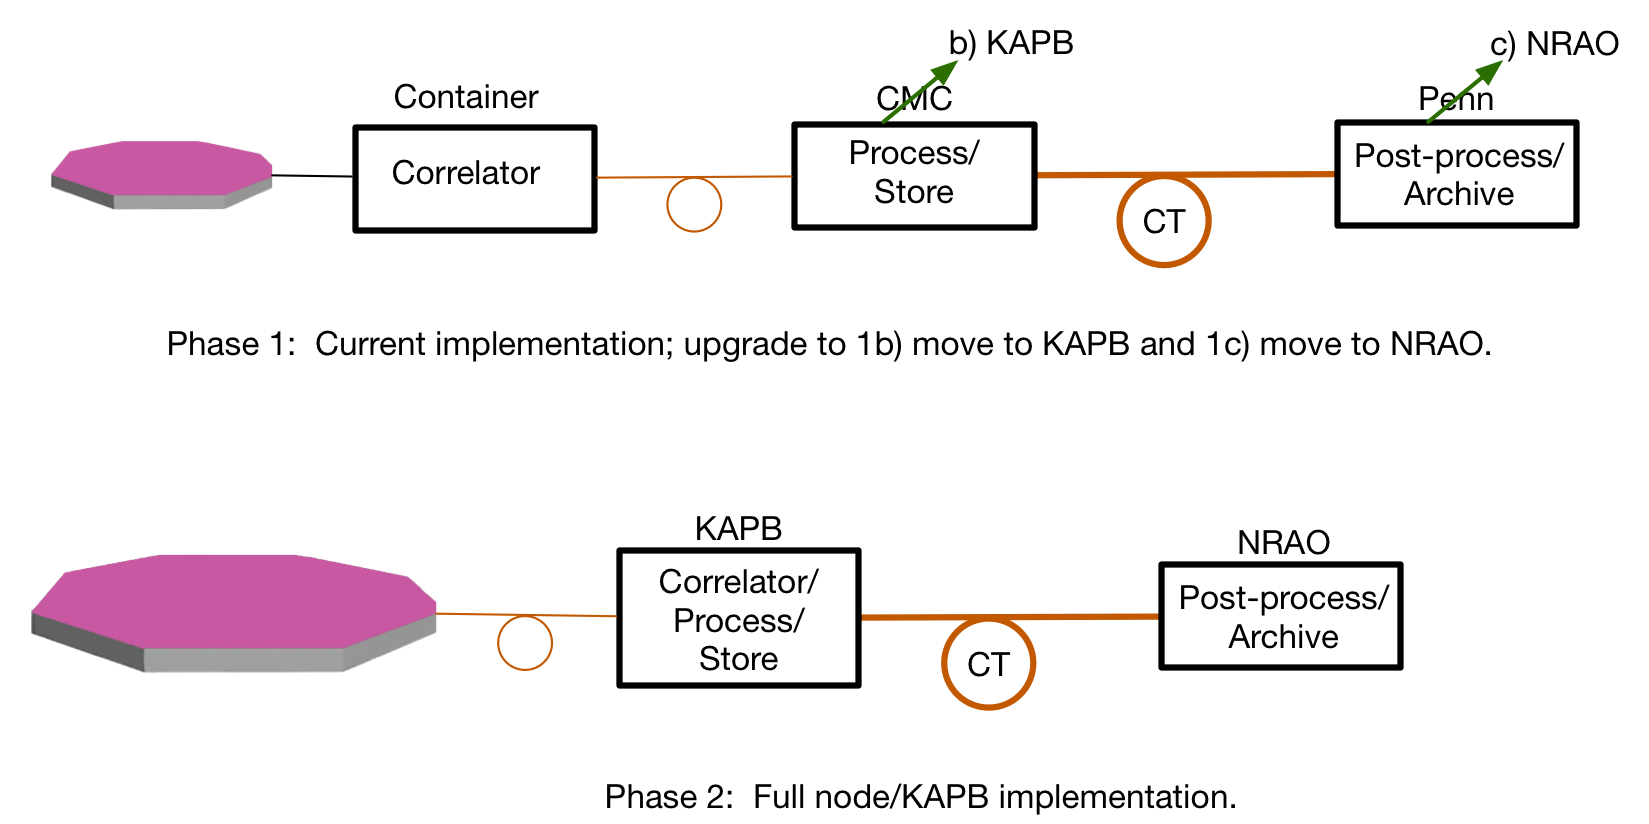
\includegraphics[width=0.75\textwidth]{bw_planning.png}
\centering
\caption{\small Phasing of the internet data links.  Top is the current phase (and indicated minor updates) while bottom is the eventual configuration.  
The link of interest is between South Africa and the US, indicated by a thick orange line.}
\label{fig:phasing}
\end{figure}

\end{document}